
\chapter{Provable Estimation Difference}\label{ch:priv_estimation}

% 
% 8888888b.  8888888b.   .d88888b.  888888b.   
% 888   Y88b 888   Y88b d88P" "Y88b 888  "88b  
% 888    888 888    888 888     888 888  .88P  
% 888   d88P 888   d88P 888     888 8888888K.  
% 8888888P"  8888888P"  888     888 888  "Y88b 
% 888        888 T88b   888     888 888    888 
% 888        888  T88b  Y88b. .d88P 888   d88P 
% 888        888   T88b  "Y88888P"  8888888P"  
%                                              
%                                              
%                                              
% 

\section{Problem Formulation}\label{sec:priv_estimation:problem}
In this chapter, we look at the problem of formalising estimation performances from a cryptographic perspective and allowing meaningful cryptographic guarantees when comparing estimators. The scenario that we will use to build this formalisation, capturing a generally applicable scenario, is one where system and measurement models are known and stochastic, and state estimators can have access to secret keys, providing them with a certain privilege. Estimators holding no keys are termed unprivileged. In addition, we will develop a single-sensor scheme that quantifies and cryptographically guarantees a difference between privileged and unprivileged estimator performances when both estimators have access to the same measurements and when models are Gaussian and linear. Further, we look at the extension to multiple sensors and the effect of fusion on cryptographic estimation performance guarantees as well as the applicability of the method to non-linear models.

To capture the aim of comparing a privileged and unprivileged estimator, we first define how to assess the estimation difference between them, and which algorithms are required to characterise a privileged estimation scheme. After giving relevant formal cryptographic definitions, the considered single-sensor privileged estimation problem and its extension to multiple sensors are presented.

% 
%  ######  ########  ##    ## ########  ########  #######     ########  ########   #######  ########  
% ##    ## ##     ##  ##  ##  ##     ##    ##    ##     ##    ##     ## ##     ## ##     ## ##     ## 
% ##       ##     ##   ####   ##     ##    ##    ##     ##    ##     ## ##     ## ##     ## ##     ## 
% ##       ########     ##    ########     ##    ##     ##    ########  ########  ##     ## ########  
% ##       ##   ##      ##    ##           ##    ##     ##    ##        ##   ##   ##     ## ##     ## 
% ##    ## ##    ##     ##    ##           ##    ##     ##    ##        ##    ##  ##     ## ##     ## 
%  ######  ##     ##    ##    ##           ##     #######     ##        ##     ##  #######  ########  
% 

\subsection{Formal Cryptographic Problem}\label{subsec:priv_estimation:crypto_problem}
While we later introduce assumptions on the system and measurement models, it is more practical to define a broader security notion that can be satisfied under arbitrary specified conditions on the models. This lends the use of the notion to future literature and is more in line with typical cryptographic practice.

We aim to give the security notion in terms of probabilistic polynomial-time (PPT) attackers and capture the desired leakage as well as attacker capabilities. The most commonly desired leakage, cryptographic indistinguishability, is not suitable for our scenario due to our desire for both estimators to gain \textit{some} information from measurements. Instead, we define security in terms of a time series of semi-definite matrices, given arbitrary known models, such that the difference in estimation error covariances between the estimators with and without access to a privilege, respectively, is bounded by the series at all times.

To formalize this, we introduce the following notations and definitions. We assume the existence of an arbitrary process (not necessarily Gaussian or linear) following a known system model exactly, with the state at timestep $k$ denoted by $\vec{x}_k\in\mathbb{R}^d$ and model parameters $\mathcal{M}_{\mathsf{S}}$. Similarly, we assume the existence of a means of process measurement following a known measurement model exactly, with the measurement at timestep $k$ denoted by $\vec{z}_k\in\mathbb{R}^m$ and model parameters $\mathcal{M}_{\mathsf{M}}$. We can now define a relevant scheme.
\begin{definition}
    A \textit{privileged estimation scheme} is a pair of probabilistic algorithms $(\mathsf{Setup},\mathsf{Noise})$, given by
    \begin{description}
        \item[$\mathsf{Setup}(\mathcal{M}_{\mathsf{S}}, \mathcal{M}_{\mathsf{M}}, \kappa)$] On the input of models $\mathcal{M}_{\mathsf{S}}$ and $\mathcal{M}_{\mathsf{M}}$, and the security parameter $\kappa$, public parameters $\mathsf{pub}$ and a secret key $\mathsf{sk}_{\mathsf{g}}$ are created.
        \item[$\mathsf{Noise}(\mathsf{pub}, \mathsf{sk}_{\mathsf{g}}, k, \mathcal{M}_{\mathsf{S}}, \mathcal{M}_{\mathsf{M}}, \vec{z}_1, \dots, \vec{z}_k)$] On input of public parameters $\mathsf{pub}$, secret key $\mathsf{sk}_{\mathsf{g}}$, timestep $k$, models $\mathcal{M}_{\mathsf{S}}$ and $\mathcal{M}_{\mathsf{M}}$, and measurements $\vec{z}_1,\dots,\vec{z}_k$, a privileged and unprivileged modified measurement (with no required model constraints) are returned, $\vec{z}_k^{\{\mathsf{p}\}}$ and $\vec{z}_k^{\{\mathsf{up}\}}$, respectively.
    \end{description}
\end{definition}
In addition to the scheme above, we also give the following definitions to help formalize our desired security notion.
\begin{definition}\label{def:priv_estimation:crypto_estimator}
    An \textit{estimator} is any probabilistic algorithm that produces a guess of the state $\vec{x}_k$ for a given timestep $k$.
\end{definition}
\begin{definition}\label{def:priv_estimation:negligible_covariance}
    A \textit{negligible covariance function},
    \begin{equation}
        \mathsf{neglCov}_m(\kappa):\mathbb{N}\rightarrow \mathbb{R}^{m\times m}\,,
    \end{equation}
    is a function that returns a matrix $\mat{A}$ such that $\mat{A}$ is a valid covariance ($\mat{A}\succ 0$ and $\mat{A}=\mat{A}^\top$) and for each of its eigenvalues $a\in\mathsf{eig}(\mat{A})$, there exists a negligible function \cite[Def. 3.4]{katzIntroductionModernCryptography2008} $\eta$ such that $a\leq\eta(\kappa)$.
\end{definition}

Now we can give the security notion that captures the formal requirements of the estimation difference we want to capture.
\begin{definition}\label{def:priv_estimation:covariance_privilege_notion}
    A privileged estimation scheme meets the notion \textit{$\{\mat{D}_1,\mat{D}_2,\dots\}$-Covariance Privilege for Models $\mathcal{M}_{\mathsf{S}}$ and $\mathcal{M}_{\mathsf{M}}$} if for any PPT estimator $\mathcal{A}$, there exists a PPT estimator $\mathcal{A}^\prime$, such that
    \begin{equation}\label{eq:priv_estimation:covariance_privilege}
        \begin{split}
            &\mathsf{Cov}\left[\mathcal{A}\left(k, \kappa, \mathsf{pub}, \mathcal{M}_S, \mathcal{M}_M, \vec{z}_1^{\{\mathsf{up}\}},\dots,\vec{z}_k^{\{\mathsf{up}\}}\right) - \vec{x}_k \right]\\
            &-\mathsf{Cov}\left[\mathcal{A}^\prime\left(k, \kappa, \mathsf{pub}, \mathcal{M}_S, \mathcal{M}_M, \vec{z}_1^{\{\mathsf{p}\}},\dots,\vec{z}_k^{\{\mathsf{p}\}}\right) - \vec{x}_k \right]\\
            &\quad\succeq \mat{D}_k - \mathsf{neglCov}_m(\kappa)
        \end{split}
    \end{equation}
   for all $k>0$, some negligible covariance function and where matrices $\mat{D}_k$ are semi-definite, that is, $\mat{D}_k\preceq 0$ or $\mat{D}_k\succeq 0$. Here, estimators $\mathcal{A}$ and $\mathcal{A}^\prime$ are running in polynomial-time with respect to the security parameter $\kappa$, and all probabilities are taken over randomness introduced in models $\mathcal{M}_{\mathsf{S}}$ and $\mathcal{M}_{\mathsf{M}}$, estimators $\mathcal{A}$ and $\mathcal{A}^\prime$, and algorithms $\mathsf{Setup}$ and $\mathsf{Noise}$.
\end{definition}

Informally, the above definition states that no estimator that can only access unprivileged measurements $\vec{z}_1^{\{\mathsf{up}\}},\dots,\vec{z}_k^{\{\mathsf{up}\}}$ can estimate a state $\vec{x}_k$ for a timestep $k$ with an MSE covariance less than an equivalent estimator with access to privileged measurements $\vec{z}_1^{\{\mathsf{p}\}},\dots,\vec{z}_k^{\{\mathsf{p}\}}$, by a margin of at least $\mat{D}_k$. We also note that by taking probabilities over randomness introduced in the system model, and therefore the possible true states $\vec{x}_k$, the definition fits a Bayesian interpretation of probability for any stochastic system model.

% 
% ########  ######  ########    ########  ########   #######  ########  
% ##       ##    ##    ##       ##     ## ##     ## ##     ## ##     ## 
% ##       ##          ##       ##     ## ##     ## ##     ## ##     ## 
% ######    ######     ##       ########  ########  ##     ## ########  
% ##             ##    ##       ##        ##   ##   ##     ## ##     ## 
% ##       ##    ##    ##       ##        ##    ##  ##     ## ##     ## 
% ########  ######     ##       ##        ##     ##  #######  ########  
% 

\subsection{Estimation Problem}\label{subsec:priv_estimation:estimation_problem}
To make use of the introduced cryptographic notion, we consider specific estimation models to use in the single-sensor case when developing a privileged estimation scheme with a provable estimation performance difference between privileged and unprivileged estimators. A system model gives the state $\vec{x}_k\in\mathbb{R}^d$ at an integer timestep $k$ and is given by
\begin{equation}\label{eq:priv_estimation:system_model}
    \vec{x}_k = \mat{F}_k\vec{x}_{k-1} + \vec{w}_k\,,
\end{equation}
with noise term $\vec{w}_k\sim \mathcal{N}(\vec{0}, \mat{Q}_k)$ and a known non-zero covariance $\mat{Q}_k\in \mathbb{R}^{d\times d}$. Similarly, the measurement model gives a measurement $\vec{z}_k$ at a timestep $k$ and is given by
\begin{equation}\label{eq:priv_estimation:single_sensor_measurement_model}
    \vec{z}_k = \mat{H}_k\vec{x}_k + \vec{v}_k\,,
\end{equation}
with noise term $\vec{v}_k\sim \mathcal{N}(\vec{0}, \mat{R}_k)$ and a known non-zero covariance $\mat{R}_k\in \mathbb{R}^{m\times m}$.

In this scenario, the sensor holds a secret key $\mathsf{sk}_{\mathsf{g}}$ that it uses to modify its measurements, and privileged estimators hold this shared key while unprivileged estimators do not. We also assume that sensors and estimators are synchronised in timestep $k$ to simplify later cryptographic evaluation.

% 
% ######## ##     ##  ######     ########  ########   #######  ########  
% ##       ##     ## ##    ##    ##     ## ##     ## ##     ## ##     ## 
% ##       ##     ## ##          ##     ## ##     ## ##     ## ##     ## 
% ######   ##     ##  ######     ########  ########  ##     ## ########  
% ##       ##     ##       ##    ##        ##   ##   ##     ## ##     ## 
% ##       ##     ## ##    ##    ##        ##    ##  ##     ## ##     ## 
% ##        #######   ######     ##        ##     ##  #######  ########  
% 

\subsection{Multi-Sensor Problem}\label{subsec:priv_estimation:fusion_problem}
As well as the single-sensor problem, we are also interested in the extension to environments with multiple sensors, where the fusion of measurements can also lead to better estimation performance irrespective of privilege. Here, we only consider multiple privileges, such that estimators with a higher privilege should perform better than those with a lower one while taking into consideration the estimation benefits from fusing additional measurements. We again consider linear and Gaussian models, where the state $\vec{x}_k \in \mathbb{R}^d$ follows the system model \eqref{eq:priv_estimation:system_model}. Measurements $\vec{z}_{k,i} \in \mathbb{R}^m$ are now indexed by sensor $i$, $1\leq i\leq n$, and follow the measurement models
\begin{equation}\label{eq:priv_estimation:multi_sensor_measurement_models}
    \vec{z}_{k,i} = \mat{H}_{k,i} \vec{x}_k + \vec{v}_{k,i}\,,
\end{equation}
with noise terms $\vec{v}_{k,i} \sim \mathcal{N}(\vec{0},\mat{R}_{k,i})$ and known non-zero covariances $\mat{R}_{k,i} \in \mathbb{R}^{m \times m}$. In addition to these models, we again assume synchronisation, between all estimators and sensors $i$, in timesteps $k$, simplifying later cryptographic evaluation.

In this scenario, each sensor holds its own secret key $\mathsf{sk}_{\mathsf{g}, i}$, $1\leq i\leq n$, which is shared with estimators of appropriate privileges. The privileges that we consider, in terms of access to keys and measurements, will be defined by sequential sensor access. That is, in the presence of $n$ sensors, we will consider exactly $n$ possible privilege levels, where each privilege $\pi>0$ corresponds to holding the sequential secret keys $\mathsf{sk}_{\mathsf{g},j}$, $1\leq j\leq \pi$, while being unprivileged, $\pi=0$, corresponds to holding none. Additionally, we assume that estimators have access to all privileged measurements, those from sensors whose keys they hold, but can fuse additional unprivileged measurements, from those whose keys they do not hold. To simplify notation, we consider access to unprivileged measurements to be sequential as well, and can therefore capture estimator capabilities by letting $\mathsf{e}^{[\pi,\tau]}$ denote an estimator with privilege $\pi$ and access to measurements from $\tau\geq\pi$ sensors $i$, $1\leq i\leq \tau$.

Multiple measurements and the effects of privilege and fusion on estimation performance complicate the cryptographic analysis in the case of multiple sensors. To demonstrate that a presented scheme guarantees better performance for higher privilege estimators while limiting the benefit from fusing unprivileged measurements, the covariance privilege notion in section \ref{subsec:priv_estimation:crypto_problem} will be used to guarantee two estimation performance differences for each privilege $\pi$.
\begin{description}
    \item[Performance Loss Lower Bound (PLLB)] Here, we aim to guarantee a lower bound on the estimation performance loss of any unprivileged estimator $\mathsf{e}^{[0, n]}$ on a privilege-$\pi$ estimator $\mathsf{e}^{[\pi,\pi]}$. Naturally, this will remain a lower bound when unprivileged estimators have access to fewer unprivileged measurements or privileged estimators have access to more.
    \item[Performance Gain Upper Bound (PGUB)] This bound will guarantee an upper bound on the estimation performance gain of any estimator $\mathsf{e}^{[\pi, n]}$ on a privilege-$\pi$ estimator $\mathsf{e}^{[\pi,\pi]}$. The bound similarly remains an upper bound when fewer unprivileged measurements are fused.
\end{description}
Lastly, a suitable scheme should be one with at least two free parameters responsible for controlling the values of these two bounds.
\begin{remark}
  We stress that the two bounds that will be guaranteed only bound the performances of estimators of the specified forms. That is, nothing is said about estimators which may corrupt sensors to obtain keys beyond their privilege or additional unprivileged measurements. Bounds on leakage caused by corrupting sensors can in some cases be captured by estimators of a new form $\mathsf{e}^{[\pi^\prime,\tau^\prime]}$, but are in general beyond the scope of this thesis.
\end{remark}


% 
% 8888888b.  8888888b.  8888888 888     888      8888888888 .d8888b. 88888888888 
% 888   Y88b 888   Y88b   888   888     888      888       d88P  Y88b    888     
% 888    888 888    888   888   888     888      888       Y88b.         888     
% 888   d88P 888   d88P   888   Y88b   d88P      8888888    "Y888b.      888     
% 8888888P"  8888888P"    888    Y88b d88P       888           "Y88b.    888     
% 888        888 T88b     888     Y88o88P        888             "888    888     
% 888        888  T88b    888      Y888P         888       Y88b  d88P    888     
% 888        888   T88b 8888888     Y8P          8888888888 "Y8888P"     888     
%                                                                                
%                                                                                
%                                                                                
% 

\section{Privileged Estimation for Linear Systems}\label{sec:priv_estimation:privileged_estimation}
In this section, we propose a privileged estimation scheme meeting the security notion in section \ref{subsec:priv_estimation:crypto_problem} for a derivable series of semi-definite matrices when models $\mathcal{M}_{\mathsf{S}}$ and $\mathcal{M}_{\mathsf{M}}$ are given by \eqref{eq:priv_estimation:system_model} and \eqref{eq:priv_estimation:single_sensor_measurement_model}, respectively. The key idea behind the method is to add pseudorandom Gaussian noise to existing measurement noise at the sensor, degrading estimation at estimators that cannot remove it. This added noise is a keystream generated by the sensor's secret key and can only be removed from measurements by an estimator holding the same key.

% 
% ##    ## ######## ##    ##  ######  ######## ########  ########    ###    ##     ## 
% ##   ##  ##        ##  ##  ##    ##    ##    ##     ## ##         ## ##   ###   ### 
% ##  ##   ##         ####   ##          ##    ##     ## ##        ##   ##  #### #### 
% #####    ######      ##     ######     ##    ########  ######   ##     ## ## ### ## 
% ##  ##   ##          ##          ##    ##    ##   ##   ##       ######### ##     ## 
% ##   ##  ##          ##    ##    ##    ##    ##    ##  ##       ##     ## ##     ## 
% ##    ## ########    ##     ######     ##    ##     ## ######## ##     ## ##     ## 
% 

\subsection{Gaussian Keystream}\label{subsec:priv_estimation:est_gaussian_keystream}
To generate the desired pseudorandom Gaussian noise that can be added to existing measurements, the sensor first generates a typical cryptographic pseudorandom bitstream with its secret key $\mathsf{sk}_{\mathsf{g}}$. This can be done with any cryptographic stream cipher and reduces the security of the method to a single, well-studied and replaceable component. This bitstream can be interpreted as sequential pseudorandom integers of a suitable size and used to generate a sequence of pseudorandom uniform real numbers $\upsilon_t\ \dot{\sim}\ \mathcal{U}(0,1)$ for sequence indices $t>0$.

Here, we note that the conversion to real numbers $\upsilon_t$ is cryptographically non-trivial due to floating-point representation affecting the pseudorandomness of the samples, and complicating the meeting of a desired cryptographic notion. Instead, we assume that floating-point numbers are sufficiently close to real numbers and rely on any common method for choosing the bit size of pseudorandom integers and the generation of uniform numbers $\upsilon_t$ \cite{goualardGeneratingRandomFloatingPoint2020}. This assumption will be further discussed with the security of the presented scheme in section \ref{subsec:priv_estimation:est_security}.

With this assumption, we are left with generating a series of pseudorandom standard Gaussian samples, which can be readily computed using the Box-Muller transform \cite{paleyFourierTransformsComplex1934}. This is given by
\begin{equation}
    \psi_t = \sqrt{-2\ln (\upsilon_t)}\cos(2\pi \upsilon_{t+1})
\end{equation}
and
\begin{equation}
    \psi_{t+1} = \sqrt{-2\ln (\upsilon_t)}\sin(2\pi \upsilon_{t+1})\,,
\end{equation}
obtaining two, independent, standard Gaussian samples from two uniform ones. To generate noise that can be added by the sensor and removed by a privileged estimator using this series, a conversion to a $d$-dimension zero-mean multivariate Gaussian sample is required at every timestep $k$. As control over the difference in estimation error between privileged and unprivileged estimators is desired, a symmetric matrix parameter $\mat{S}\succ 0$ is introduced, such that added pseudorandom noise $\vec{g}_k$ follows distribution $\vec{g}_k\ \dot{\sim}\ \mathcal{N}(\vec{0},\mat{S})$. Given $\mat{S}$, $\vec{g}_k$ can be computed using the next $d$ Gaussian keystream samples,
\begin{equation}\label{eq:priv_estimation:est_gaussian_standard_noise_stream}
    \vec{\psi}_k =
    \begin{bmatrix}
        \psi_{(k-1)d+1} & \dots & \psi_{kd}
    \end{bmatrix}^\top\,,
\end{equation}
as
\begin{equation}\label{eq:priv_estimation:est_gaussian_noise_stream}
    \vec{g}_k = \mat{S}^{\frac{1}{2}}\vec{\psi}_k
\end{equation}
for any matrix $\mat{S}^{\frac{1}{2}}$ such that $\mat{S}^{\frac{1}{2}}\mat{S}^{\frac{1}{2}\top}=\mat{S}$. We also note that for the correct removal of noise terms $\vec{g}_k$ by the privileged estimator, index information $k$ is required but available when sensors and estimators are synchronised, as assumed in our case.

% 
% ##     ##  #######  ########  
% ###   ### ##     ## ##     ## 
% #### #### ##     ## ##     ## 
% ## ### ## ##     ## ##     ## 
% ##     ## ##     ## ##     ## 
% ##     ## ##     ## ##     ## 
% ##     ##  #######  ########  
% 

\subsection{Measurement Modification}\label{subsec:priv_estimation:est_measurement_mod}
Using the noise in \eqref{eq:priv_estimation:est_gaussian_noise_stream}, the sensor can now modify measurements $\vec{z}_k$ by
\begin{equation}\label{eq:priv_estimation:est_modified_measurement}
    \vec{z}^\prime_k = \vec{z}_k + \vec{g}_k\,,
\end{equation}
resulting in a new measurement model
\begin{equation}
    \vec{z}^\prime_k = \mat{H}_k\vec{x}_k + \vec{v}_k + \vec{g}_k\,,
\end{equation}
with noise terms $\vec{v}_k\sim \mathcal{N}(\vec{0},\mat{R}_k)$ and $\vec{g}_k\ \dot{\sim}\ \mathcal{N}(\vec{0},\mat{S})$. This leads to two estimation problems for the privileged and unprivileged estimators, respectively.
\begin{description}
    \item[Privileged estimation] An estimator that holds the secret key $\mathsf{sk}_{\mathsf{g}}$ can compute the Gaussian key stream $\psi_t$, $t>0$, and therefore the added noise vectors $\vec{g}_k$ at every timestep $k$. Given the modified measurements \eqref{eq:priv_estimation:est_modified_measurement}, computing $\vec{z}_k = \vec{z}^\prime_k - \vec{g}_k$  obtains measurements following the measurement model \eqref{eq:priv_estimation:single_sensor_measurement_model} exactly.
    \item[Unprivileged estimation] In the case where pseudorandomness is indistinguishable from randomness, as is the case for an unprivileged estimator when a cryptographically secure keystream is used and the secret key $\mathsf{sk}_{\mathsf{g}}$ is not known, modified measurements are indistinguishable from those following the unprivileged measurement model 
    \begin{equation}\label{eq:priv_estimation:est_unpriv_measurement_model}
        \vec{z}^\prime_k = \mat{H}_k\vec{x}_k + \vec{v}^\prime_k\,,
    \end{equation}
   with $\vec{v}^\prime_k\sim \mathcal{N}(\vec{0},\mat{R}_k+\mat{S})$, exactly.
\end{description}

Intuitively, we can see that the two types of estimators have the difference between their estimation errors dependent on matrix $\mat{S}$.

% 
%  ######  ########  ######  
% ##    ## ##       ##    ## 
% ##       ##       ##       
%  ######  ######   ##       
%       ## ##       ##       
% ##    ## ##       ##    ## 
%  ######  ########  ######  
% 

\subsection{Security Analysis}\label{subsec:priv_estimation:est_security}
Recalling definition \ref{def:priv_estimation:covariance_privilege_notion}, we aim to show how the notion is met by the proposed estimation scheme. Before the proof sketch, we look at our scheme in the context of a formal privileged estimation scheme with model constraints and give some relevant optimality properties.

We consider the stochastic system model \eqref{eq:priv_estimation:system_model} and measurement model \eqref{eq:priv_estimation:single_sensor_measurement_model} exactly, that is, any linear models with known covariance, zero-mean, Gaussian additive noises. We define these as our model conditions and capture all relevant parameters in the respective equations in $\mathcal{M}_{\mathsf{S}}$ and $\mathcal{M}_{\mathsf{M}}$. Our scheme meets the definition of a formal privileged estimation scheme by defining the required algorithms $\mathsf{Setup}$ and $\mathsf{Noise}$ as
\begin{description}
    \item[$\mathsf{Setup}(\mathcal{M}_{\mathsf{S}}, \mathcal{M}_{\mathsf{M}}, \kappa)$] Initialize a cryptographically indistinguishable stream cipher with the parameter $\kappa$, set the secret key $\mathsf{sk}_{\mathsf{g}}$ to the stream cipher key and include an initial filter estimate $\hat{\vec{x}}_0$, error covariance $\mat{P}_0$ and added noise covariance $\mat{S}$ in the public parameters $\mathsf{pub}$.
    \item[$\mathsf{Noise}(\mathsf{pub}, \mathsf{sk}_{\mathsf{g}}, k, \mathcal{M}_{\mathsf{S}}, \mathcal{M}_{\mathsf{M}}, \vec{z}_1, \dots, \vec{z}_k)$] Using the stream cipher key $\mathsf{sk}_{\mathsf{g}}$ and public parameters $\mathsf{pub}$, create an unprivileged measurement by \eqref{eq:priv_estimation:est_modified_measurement}. Set and return the privileged measurement $\vec{z}^{\{\mathsf{p}\}}_k=\vec{z}_k$ and unprivileged measurement $\vec{z}^{\{\mathsf{up}\}}_k=\vec{z}^\prime_k$.
\end{description}
Here, we note that in the $\mathsf{Setup}$ algorithm above, the inclusion of an initial state estimate, its error covariance and the generated noise covariance in the public parameters $\mathsf{pub}$ are present only for the completeness of the cryptographic definition and not a requirement for the security of the scheme.

The idea behind our proof sketch relies on the optimality of the linear KF introduced in section \ref{subsec:prelims:kf_opt}. Given an initial estimate and its error covariance, the KF produces updated estimates with the minimum MSE achievable for \textit{any} estimator when all measurements $\vec{z}_1,\dots,\vec{z}_k$ are observed, models are Gaussian and linear, and the same initialization is used. Since the KF also preserves the initial error covariance order,
\begin{equation}
   \mat{P}_k \preceq \mat{P}_k^\prime \implies \mat{P}_{k+1} \preceq \mat{P}_{k+1}^\prime\,,
\end{equation}
for two different filter estimate error covariances $\mat{P}_k$ and $\mat{P}_k^\prime$, we can define an error covariance lower-bound $\mat{P}_k^{(l)}$ for all possible initialisations by setting $\mat{P}_0^{(l)} = \mat{0}$ and computing the KF error covariance using the combined predict and update equations
\begin{equation}\label{eq:priv_estimation:est_lower_bound_error_cov}
    \begin{split}
        \mat{P}_k^{(l)} =& \Bigl( \mat{I} - (\mat{F}_k\mat{P}_{k-1}^{(l)}\mat{F}_k^\top + \mat{Q}_k)\mat{H}_k^\top \bigl(\mat{H}_k(\mat{F}_k\mat{P}_{k-1}^{(l)}\mat{F}_k^\top + \mat{Q}_k)\mat{H}_k^\top + \mat{R}_k\bigr)^{-1}\mat{H}_k\Bigr)\cdot\\
        &\quad\Bigl(\mat{F}_k\mat{P}_{k-1}^{(l)}\mat{F}_k^\top + \mat{Q}_k\Bigr)\,.
    \end{split}
\end{equation}
This gives us a lower bound at every timestep $k$, such that
\begin{equation}
    \mat{P}_k^{(l)} \preceq \mathsf{Cov}\left[\mathcal{A}\left(k, \mathcal{M}_{\mathsf{S}}, \mathcal{M}_{\mathsf{M}}, \vec{z}_1,\dots,\vec{z}_k\right) - \vec{x}_k \right]
\end{equation}
for \textit{any} estimator $\mathcal{A}$ following definition \ref{def:priv_estimation:crypto_estimator} and any Gaussian and linear models $\mathcal{M}_{\mathsf{S}}$ and $\mathcal{M}_{\mathsf{M}}$. This leads us to the proof sketch.

% 
% .########..########...#######...#######..########
% .##.....##.##.....##.##.....##.##.....##.##......
% .##.....##.##.....##.##.....##.##.....##.##......
% .########..########..##.....##.##.....##.######..
% .##........##...##...##.....##.##.....##.##......
% .##........##....##..##.....##.##.....##.##......
% .##........##.....##..#######...#######..##......
% 

\subsubsection{Proof Sketch}
We wish to show that the scheme in section \ref{subsec:priv_estimation:est_measurement_mod} meets $\{\mat{D}_1,\mat{D}_2,\dots\}$-Covariance Privilege for Models $\mathcal{M}_{\mathsf{S}}$ and $\mathcal{M}_{\mathsf{M}}$, for a computable series $\mat{D}_k$, $k>0$ dependent on a noise parameter $\mat{S}$, when $\mathcal{M}_{\mathsf{S}}$ and $\mathcal{M}_{\mathsf{M}}$ are Gaussian and linear. 

Since a cryptographically pseudorandom stream cipher is used, the stream integers, and therefore the uniform samples $\upsilon_t$ and Gaussian samples $\psi_t$, are indistinguishable from those generated from a truly random stream for any PPT estimator without the secret key. We persist with the previous assumption that floating-point representations of $\psi_t$ are sufficiently close to Gaussian and assume the KF to provide optimal estimation when using floating-point arithmetic. Using the $\mathsf{Setup}$ and $\mathsf{Noise}$ algorithms given in section \ref{subsec:priv_estimation:est_security} leads to pseudorandom measurements $\vec{z}^\prime_k$ that are indistinguishable from measurements following the unprivileged measurement model \eqref{eq:priv_estimation:est_unpriv_measurement_model}. We can then compute a lower-bound $\mat{P}_k^{\prime(l)}$ for any unprivileged estimator as $\mat{P}_0^{\prime(l)}=\mat{0}$ and
\begin{equation}\label{eq:priv_estimation:est_unprivileged_lower_bound_error_cov}
   \begin{split}
      \mat{P}_k^{\prime(l)} =& \Bigl( \mat{I} - (\mat{F}_k\mat{P}_{k-1}^{\prime(l)}\mat{F}_k^\top + \mat{Q}_k)\mat{H}_k^\top\bigl(\mat{H}_k(\mat{F}_k\mat{P}_{k-1}^{\prime(l)}\mat{F}_k^\top + \mat{Q}_k)\mat{H}_k^\top + \mat{R}_k+\mat{S}\bigr)^{-1}\mat{H}_k\Bigr)\cdot\\
      &\quad\Bigl(\mat{F}_k\mat{P}_{k-1}^{\prime(l)}\mat{F}_k^\top + \mat{Q}_k\Bigr)\,.
   \end{split}
\end{equation}
Taking the difference of \eqref{eq:priv_estimation:est_unprivileged_lower_bound_error_cov} and the lower bound error covariances for privileged estimators \eqref{eq:priv_estimation:est_lower_bound_error_cov} produces the series
\begin{equation}\label{eq:priv_estimation:est_covariance_difference_series}
   \mat{D}_k = \mat{P}_k^{\prime(l)} - \mat{P}_k^{(l)}\,,
\end{equation}
for $k>0$, which can be tuned by the parameter $\mat{S}$. Since both series $\mat{P}_k^{(l)}$ and $\mat{P}_k^{\prime(l)}$ give the lowest possible error covariance of the respective estimators, an estimator following the true model \eqref{eq:priv_estimation:single_sensor_measurement_model} can always be created for one following the unprivileged model \eqref{eq:priv_estimation:est_unpriv_measurement_model} such that their error covariances differ by at least $\mat{D}_k$ for each timestep $k$. A reduction proof can therefore be constructed, in which the existence of an unprivileged estimator that produces estimates such that \eqref{eq:priv_estimation:covariance_privilege} does not hold, implies the existence of an estimator with an error covariance lower than $\mat{P}_k^{\prime(l)}$ following model \eqref{eq:priv_estimation:est_unpriv_measurement_model}. As no such estimator exists, we conclude that our scheme meets $\{\mat{D}_1,\mat{D}_2,\dots\}$-Covariance Privilege for Models $\mathcal{M}_S$ and $\mathcal{M}_M$, when models are Gaussian and linear, concluding our proof sketch.

% 
% ....###.....######...######..##.....##.##.....##.########.
% ...##.##...##....##.##....##.##.....##.###...###.##.....##
% ..##...##..##.......##.......##.....##.####.####.##.....##
% .##.....##..######...######..##.....##.##.###.##.########.
% .#########.......##.......##.##.....##.##.....##.##.......
% .##.....##.##....##.##....##.##.....##.##.....##.##.......
% .##.....##..######...######...#######..##.....##.##.......
% 

\subsubsection{Implicit Assumptions}
In addition to the proof sketch, we stress some comments on accepting cryptographic guarantees in terms of estimation models $\mathcal{M}_{\mathsf{S}}$ and $\mathcal{M}_{\mathsf{M}}$ when used to estimate a physical process or approximate continuous models. The following assumptions are made in this scenario.
\begin{description}
    \item[Exact models] When assigning a model to a physical process, any cryptographic guarantees about the model assume it describes the process \textit{exactly}. Often, models assume a Bayesian interpretation of probability (a stochastic state) or are chosen to simplify estimation, resulting in the possibility of better estimation given alternative or more complicated models. Although the standard for state estimation, we state the assumption to highlight the distinction between models and a physical process.
    \item[Floating-point approximation] As stated in section \ref{subsec:priv_estimation:est_gaussian_keystream} and the proof sketch above, floating-point approximations to real numbers complicate cryptographic guarantees when relying on proofs using real numbers such as KF optimality. While optimal estimation with floating-point numbers is beyond the scope of this thesis, their prevalence in the field of state estimation justifies the assumption of sufficient similarity and the insignificance of associated error introduced to the security notion.
\end{description}

% 
% .##....##..#######..##....##.........##.......####.##....##
% .###...##.##.....##.###...##.........##........##..###...##
% .####..##.##.....##.####..##.........##........##..####..##
% .##.##.##.##.....##.##.##.##.#######.##........##..##.##.##
% .##..####.##.....##.##..####.........##........##..##..####
% .##...###.##.....##.##...###.........##........##..##...###
% .##....##..#######..##....##.........########.####.##....##
% 

\subsubsection{Non-Linear Systems}
As the presented scheme provides a provable performance difference between privileged and unprivileged estimators when models are Gaussian and linear, it leaves the question of what can be said about the covariance privilege notion in our scheme when models are arbitrary non-linear functions. The basis of our cryptographic guarantee is that optimal estimators for the considered models are known and therefore guarantee a certain difference between privileged and unprivileged estimators' performances. Here, we assume that models are exact but accept that the cryptographic guarantee is useful even when physical processes are not modelled perfectly, as long as optimal linear estimators exist and estimate the process sufficiently well. With this reasoning, we argue that the covariance privilege proof sketch can be similarly applied to non-linear methods when using a non-linear (and non-optimal) estimator. In this case, the difference is no longer cryptographically guaranteed, even if models were exact, since better estimators may exist. However, a derivable difference in performance between known and well-performing estimators, with access to privileged and unprivileged measurements, respectively, still provides meaningful and valuable security information.

% 
%  ######  #### ##     ## 
% ##    ##  ##  ###   ### 
% ##        ##  #### #### 
%  ######   ##  ## ### ## 
%       ##  ##  ##     ## 
% ##    ##  ##  ##     ## 
%  ######  #### ##     ## 
% 

\subsection{Simulation}\label{subsec:priv_estimation:est_simulation}
Simulation results of the presented privileged estimation scheme are shown here in addition to the theoretical backing above. As in previous chapters, we simulated the two-dimension time-invariant constant velocity system model,
\begin{equation}\label{eq:priv_estimation:est_simulation_system_model}
    \vec{x}_k = 
    \begin{bmatrix}
        1 & 0 & 0.5 & 0\\
        0 & 1 & 0 & 0.5\\
        0 & 0 & 1 & 0\\
        0 & 0 & 0 & 1
    \end{bmatrix}
    \vec{x}_{k-1} + \vec{w}_k\,,
\end{equation}
with noise term
\begin{equation}
    \vec{w}_k \sim \mathcal{N}\left(\vec{0},\ \frac{1}{10^{3}}\cdot
    \begin{bmatrix}
        0.42 & 0 & 1.25 & 0\\
        0 & 0.42 & 0 & 1.25\\
        1.25 & 0 & 5.0 & 0\\
        0 & 1.25 & 0 & 5.0
    \end{bmatrix}
    \right)\,.
\end{equation}
Two measurement models were considered, with bounded and unbounded system errors, respectively, and estimators were implemented using the linear KF with initial error covariance $\mat{0}$. Simulations were written in the Python programming language and the AES block cipher in counter mode (AES-CTR) \cite{gueronIntelAdvancedEncryption2010} was used as the cryptographically secure stream cipher.

The first measurement model measured state location, leading to an asymptotically stable system with bounded error covariances as $k \rightarrow \infty$. It was given by 
\begin{equation}\label{eq:priv_estimation:est_simulation_measurement_model_bounded}
    \vec{z}_k=
    \begin{bmatrix}
        1 & 0 & 0 & 0\\
        0 & 1 & 0 & 0
    \end{bmatrix}
    \vec{x}_k + \vec{v}_k
\end{equation}
and
\begin{equation}
    \vec{v}_k \sim \mathcal{N}\left(\vec{0},
    \begin{bmatrix}
        5 & 2\\
        2 & 5
    \end{bmatrix}\right)\,.
\end{equation}
The sensor added pseudorandom Gaussian samples with a covariance $\mat{S}=35 \cdot \mat{I}$ according to our scheme in section \ref{subsec:priv_estimation:est_measurement_mod}. Figure \ref{fig:priv_estimation:est_sim_bounded} shows the average error covariance traces and the MSE of a privileged and unprivileged estimator for $1000$ simulations runs using the models \eqref{eq:priv_estimation:est_simulation_system_model} and \eqref{eq:priv_estimation:est_simulation_measurement_model_bounded}. 
\begin{figure}[htbp]
    \centering
    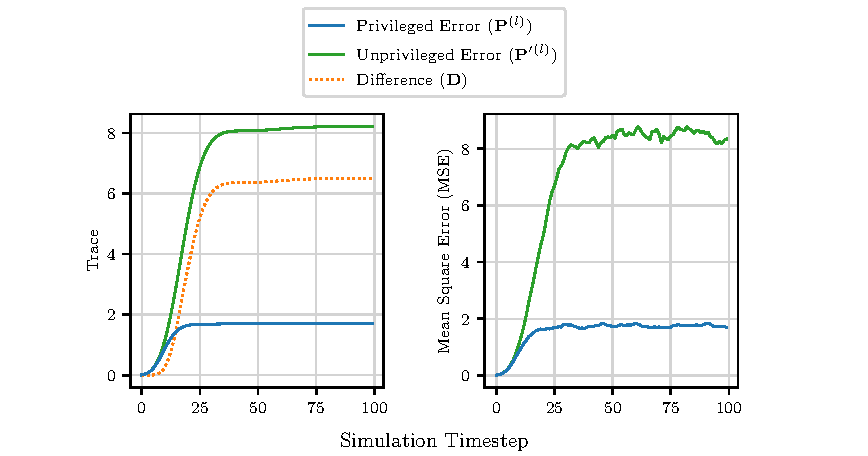
\includegraphics{figures/priv_estimation_est_sim_bounded.pdf}
    \caption{Error covariance trace and average MSE from $1000$ simulation runs with measurement model \eqref{eq:priv_estimation:est_simulation_measurement_model_bounded}}
    \label{fig:priv_estimation:est_sim_bounded}
\end{figure}
As expected, it can be seen that the privileged estimator's error covariance trace is lower than the unprivileged estimator's and that the privileged estimator has a lower MSE. The difference in trace between the two estimators has also been plotted and equals the trace of the series \eqref{eq:priv_estimation:est_covariance_difference_series} due to the simulation initial error covariance $\mat{0}$.

The second simulation considered an asymptotically unstable system where only state velocity is measured, leading to an unbounded error covariance as $k \rightarrow \infty$. It was given by 
\begin{equation}\label{eq:priv_estimation:est_simulation_measurement_model_unbounded}
    \mat{z}_k=
    \begin{bmatrix}
        0 & 0 & 1 & 0\\
        0 & 0 & 0 & 1
    \end{bmatrix}
    \vec{x}_k + \vec{v}_k\,,
\end{equation}
and the same noise distribution and keystream covariance $\mat{S}$ as in the bounded case. Figure \ref{fig:priv_estimation:est_sim_unbounded} shows the average error covariance traces and MSE of estimation from $1000$ simulation runs with models \eqref{eq:priv_estimation:est_simulation_system_model} and \eqref{eq:priv_estimation:est_simulation_measurement_model_unbounded} and shows similar results.
\begin{figure}[htbp]
    \centering
    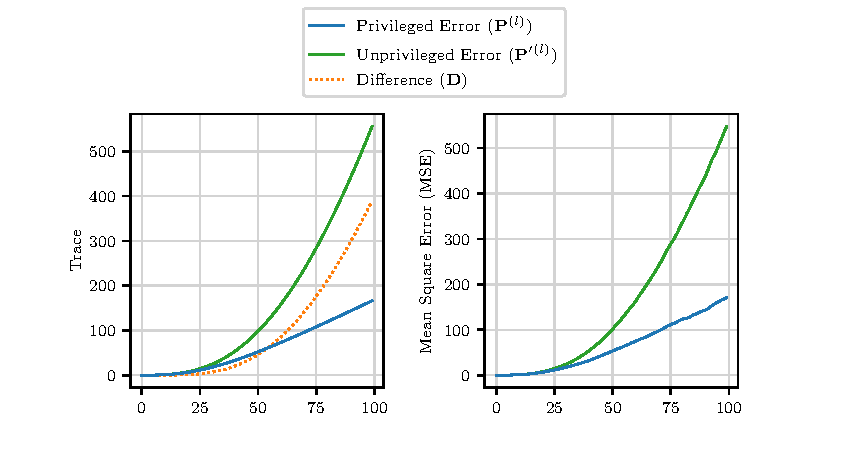
\includegraphics{figures/priv_estimation_est_sim_unbounded.pdf}
    \caption{Error covariance trace and average MSE from $1000$ simulation runs with measurement model \eqref{eq:priv_estimation:est_simulation_measurement_model_unbounded}}
    \label{fig:priv_estimation:est_sim_unbounded}
\end{figure}

Both figures capture the difference in estimation error between the best possible estimators given the simulated processes (in terms of MSE) and support the security proof sketch in section \ref{subsec:priv_estimation:est_security}.

% 
% 8888888b.  8888888b.  8888888 888     888      8888888888 888     888  .d8888b.  8888888888 
% 888   Y88b 888   Y88b   888   888     888      888        888     888 d88P  Y88b 888        
% 888    888 888    888   888   888     888      888        888     888 Y88b.      888        
% 888   d88P 888   d88P   888   Y88b   d88P      8888888    888     888  "Y888b.   8888888    
% 8888888P"  8888888P"    888    Y88b d88P       888        888     888     "Y88b. 888        
% 888        888 T88b     888     Y88o88P        888        888     888       "888 888        
% 888        888  T88b    888      Y888P         888        Y88b. .d88P Y88b  d88P 888        
% 888        888   T88b 8888888     Y8P          888         "Y88888P"   "Y8888P"  8888888888 
%                                                                                             
%                                                                                             
%                                                                                             
% 

\section{Fusion in Privileged Estimation Environments}\label{sec:priv_estimation:privileged_fusion}
Recalling the problem formulation in section \ref{subsec:priv_estimation:fusion_problem}, an effective single-sensor privileged estimation scheme leads to interest in the extension to environments with multiple sensors, where multiple privileges and accesses to measurements are possible, affecting the estimation performance of present estimators. Here, we aim to present a scheme where the PLLB and the PGUB, defined in section \ref{subsec:priv_estimation:fusion_problem}, can be derived and proved using the covariance privilege notation from definition \ref{def:priv_estimation:covariance_privilege_notion}. The idea behind the scheme is to add \textit{correlated} Gaussian keystreams to the measurements from each sensor. These noises can be computed and subtracted by estimators holding respective sensor keys, while their correlation limits the additional information gained from fusing unprivileged measurements.

% 
%  ######   #######  ########  ########     ##    ## ######## ##    ##  ######  
% ##    ## ##     ## ##     ## ##     ##    ##   ##  ##        ##  ##  ##    ## 
% ##       ##     ## ##     ## ##     ##    ##  ##   ##         ####   ##       
% ##       ##     ## ########  ########     #####    ######      ##     ######  
% ##       ##     ## ##   ##   ##   ##      ##  ##   ##          ##          ## 
% ##    ## ##     ## ##    ##  ##    ##     ##   ##  ##          ##    ##    ## 
%  ######   #######  ##     ## ##     ##    ##    ## ########    ##     ######  
% 

\subsection{Correlated Gaussian Keystreams}\label{subsec:priv_estimation:fus_gaussian_keystreams}
Similarly to the multivariate Gaussian keystream in section \ref{subsec:priv_estimation:est_gaussian_keystream}, pseudorandom samples can be correlated in this way even when generated using different stream cipher keys. To parameterise the correlation between noises at each sensor, we introduce a fully correlated component $\mat{V}\in\mathbb{R}^{m\times m}$, $\mat{V}\succ\mat{0}$, and an uncorrelated component $\mat{W}\in\mathbb{R}^{m\times m}$, $\mat{W}\succ\mat{0}$, and define a noise cross-correlation matrix for $x$ noises as $\mat{S}^{(x)} \in \mathbb{R}^{xm\times xm}$,
\begin{equation}\label{eq:priv_estimation:fus_noise_correlation_matrix}
    \mat{S}^{(x)}=
    \begin{bmatrix}
        \mat{V} & \cdots & \mat{V}\\
        \vdots & \ddots & \vdots\\
        \mat{V} & \cdots & \mat{V}\\
    \end{bmatrix}+
    \begin{bmatrix}
        \mat{W} & \mat{0} & \mat{0}\\
        \mat{0} & \ddots & \mat{0}\\
        \mat{0} & \mat{0} & \mat{W}\\
    \end{bmatrix}\,,
\end{equation}
and $\mat{S}^{(1)}=\mat{V}+\mat{W}$. Denoting generated multivariate standard Gaussian noise \eqref{eq:priv_estimation:est_gaussian_standard_noise_stream} and added Gaussian noise \eqref{eq:priv_estimation:est_gaussian_noise_stream} for sensor $i$ at timestep $k$ as $\vec{\psi}_{k, i}$ and $\vec{g}_{k, i}$, respectively, the generation of all $n$ multivariate Gaussian noises at timestep $k$, $\vec{g}_k^{(1:n)}$, can be computed. This can be done by
\begin{equation}\label{eq:priv_estimation:fus_all_correlated_noises_generation}
    \begin{split}
        \vec{g}_k^{(1:n)}&=
        \begin{bmatrix}
            \vec{g}_{k,1}\\
            \vdots\\
            \vec{g}_{k,n}
        \end{bmatrix}\\
        &=\mat{S}^{(n)\frac{1}{2}}\cdot
        \begin{bmatrix}
            \vec{\psi}_{k,1}\\
            \vdots\\
            \vec{\psi}_{k,n}
        \end{bmatrix}\,,
    \end{split}
\end{equation}
where each $\vec{\psi}_{k, i}$ is computed as $\vec{\psi}_k$ in \eqref{eq:priv_estimation:est_gaussian_standard_noise_stream} using uniform samples generated with key $\mathsf{sk}_{\mathsf{g}, i}$, and $\mat{S}^{(n)\frac{1}{2}}$ is a matrix such that $\mat{S}^{(n)\frac{1}{2}}\mat{S}^{(n)\frac{1}{2}\top}=\mat{S}^{(n)}$. Notably, as we consider sequential access to keys, it is important that the vector of the first $\pi$ noises $\vec{g}_{k, i}$, $1\leq i\leq \pi$, in \eqref{eq:priv_estimation:fus_all_correlated_noises_generation}, denoted $\vec{g}_k^{(1:\pi)}$, can be reproduced by an estimator of privilege $\pi$, holding only the keys $\mathsf{sk}_{\mathsf{g}, i}$, $1\leq i\leq \pi$. One case where this is possible is when a lower-triangular decomposition, such as the Cholesky decomposition, is used to compute $\mat{S}^{(n)\frac{1}{2}}$ from $\mat{S}^{(n)}$. Then, each correlated Gaussian sample $\vec{g}_{k,i}$ is computable from preceding standard samples $\vec{\psi}_{k,j}$, $j\leq i$ only, and the generalised noise generation equation
\begin{equation}\label{eq:priv_estimation:fus_p_correlated_noises_generation}
  \vec{g}_k^{(1:\pi)}=
  \mat{S}^{(\pi)\frac{1}{2}}\cdot
  \begin{bmatrix}
    \vec{\psi}_{k,1}\\
    \vdots\\
    \vec{\psi}_{k,\pi}
  \end{bmatrix}
\end{equation}
generates the same first $\pi$ noises $\vec{g}_k^{(1:\pi)}$ as would be obtained from \eqref{eq:priv_estimation:fus_all_correlated_noises_generation}. This is due to $\mat{S}^{(\pi)\frac{1}{2}}\in\mathbb{R}^{\pi m\times \pi m}$ equalling the top left block of matrix $\mat{S}^{(n)\frac{1}{2}}$ when using the lower-triangular decomposition.

At every timestep $k$, $\vec{g}_k^{(1:n)}$ can then be generated with \eqref{eq:priv_estimation:fus_p_correlated_noises_generation} using all $n$ keys and used to modify sensor measurements, while the subset $\vec{g}_k^{(1:\pi)}$ can be generated by estimators of privilege $\pi$ using only the keys they hold.

% 
% ##     ##  #######  ########  
% ###   ### ##     ## ##     ## 
% #### #### ##     ## ##     ## 
% ## ### ## ##     ## ##     ## 
% ##     ## ##     ## ##     ## 
% ##     ## ##     ## ##     ## 
% ##     ##  #######  ########  
% 

\subsection{Measurement Modification}\label{subsec:priv_estimation:fus_measurement_mod}
With a way to generate noises for sensors and estimators, we can introduce the means of measurement modification and the observable measurement models for different estimators in the multiple-sensor environment. Measurement modification is performed by adding noises $\vec{g}_k^{(1:n)}$ to measurements from each sensor $i$ before making them public, resulting in modified measurement equations for each sensor,
\begin{equation}\label{eq:priv_estimation:fus_modified_measurements}
    \vec{z}_{k,i}^\prime = \vec{z}_{k,i} + \vec{g}_{k, i} = \mat{H}_{k,i}\vec{x}_k + \vec{v}_{k,i} + \vec{g}_{k,i}\,,
\end{equation}
with measurement noise $\vec{v}_{k,i}\sim\mathcal{N}(\vec{0},\mat{R}_{k,i})$ and the vector of all added pseudorandom noises $\vec{g}_k^{(1:n)}\ \dot{\sim}\ \mathcal{N}(\vec{0}, \mat{S}^{(n)})$. As we assume that sensors are synchronised in $k$, we can capture the correlation between these modified measurements exactly by considering the stacked measurement model for any estimator with access to $\tau$ measurements at timestep $k$, as
\begin{equation}\label{eq:priv_estimation:fus_measurement_equation}
    \vec{z}_k^{\prime(1:\tau)} = \vec{z}_k^{(1:\tau)} + \vec{g}_k^{(1:\tau)} = \mat{H}_k^{(1:\tau)}\vec{x}_k + \vec{v}_k^{(1:\tau)} + \vec{g}_k^{(1:\tau)}\,,
\end{equation}
with $\vec{v}_k^{(1:\tau)}\sim\mathcal{N}(\vec{0},\mat{R}_k^{(1:\tau)})$ and $\vec{g}_k^{(1:\tau)}\ \dot{\sim}\ \mathcal{N}(\vec{0},\mat{S}^{(\tau)})$, where
\begin{equation*}
  \vec{z}_k^{\prime(1:\tau)}=
  \begin{bmatrix}
    \vec{z}_{k,1}^\prime\\
    \vdots\\
    \vec{z}_{k,\tau}^\prime
  \end{bmatrix},\ 
  \vec{z}_k^{(1:\tau)}=
  \begin{bmatrix}
    \vec{z}_{k,1}\\
    \vdots\\
    \vec{z}_{k,\tau}
  \end{bmatrix},\ 
  \mat{H}_k^{(1:\tau)}=
  \begin{bmatrix}
    \mat{H}_{k,1}\\
    \vdots\\
    \mat{H}_{k,\tau}\\
  \end{bmatrix}\,,
\end{equation*}
\begin{equation*}
  \vec{v}_k^{(1:\tau)}=
  \begin{bmatrix}
    \vec{v}_{k,1}\\
    \vdots\\
    \vec{v}_{k,\tau}
  \end{bmatrix},\ 
  \mat{R}_k^{(1:\tau)}=
    \begin{bmatrix}
      \mat{R}_{k,1} & \mat{0} & \mat{0}\\
      \mat{0} & \ddots & \mat{0}\\
      \mat{0} & \mat{0} & \mat{R}_{k,\tau}
    \end{bmatrix}\,
\end{equation*}
and $\mat{S}^{(\tau)} \in \mathbb{R}^{\tau m\times \tau m}$ defined by \eqref{eq:priv_estimation:fus_noise_correlation_matrix}.

Since we are using a cryptographically sound stream cipher to generate the added Gaussian keystream, the pseudorandom samples are indistinguishable from truly random ones to estimators without appropriate keys, which leads us to three observable measurement models, that is, the models that capture all the information available to an estimator exactly, for three types of mutually exhaustive estimators. Recalling the estimator notation introduced in section \ref{subsec:priv_estimation:fusion_problem}, we have
\begin{description}
    \item[Estimators of the form $\mathsf{e}^{[0,\tau]}$] Here, no keys are held by an unprivileged estimator with access to $\tau$ measurements, thus all generated noises $\vec{g}_k^{(1:\tau)}$ are indistinguishable from noises from the truly random distribution $\mathcal{N}(\vec{0}, \mat{S}^{(\tau)})$. For these estimators, we can rewrite the measurement equation \eqref{eq:priv_estimation:fus_measurement_equation} as the observed measurement model
    \begin{equation}\label{eq:priv_estimation:fus_0q_obs_measurement_model}
        \vec{z}_k^{[0,\tau]} = \mat{H}_k^{(1:\tau)}\vec{x}_k + \vec{v}_k^{\prime}\,,
    \end{equation}
    with truly Gaussian term $\vec{v}_k^{\prime} \sim \mathcal{N}(\vec{0}, \mat{R}_k^{(1:\tau)}+\mat{S}^{(\tau)})$.
  
    \item[Estimators of the form $\mathsf{e}^{[\pi,\pi]}$] Estimators with keys for all the sensors to which they have access can generate all added noises and subtract them from the received measurements. That is, $\vec{g}_k^{(1:\pi)}$ can be generated and $\vec{z}_k^{[\pi,\pi]}=\vec{z}_k^{\prime(1:\pi)}-\vec{g}_k^{(1:\pi)}$ computed to give the observed measurement model equal to receiving unmodified measurements only,
    \begin{equation}\label{eq:priv_estimation:fus_pp_obs_measurement_model}
        \vec{z}_k^{[\pi,\pi]} = \mat{H}_k^{(1:\pi)}\vec{x}_k + \vec{v}_k^{(1:\pi)}\,,
    \end{equation}
    where $\vec{v}_k^{(1:\pi)} \sim \mathcal{N}(\vec{0}, \mat{R}_k^{(1:\pi)})$.

    \item[Estimators of the form $\mathsf{e}^{[\pi,\tau]}$, $\pi<\tau$] Lastly, we want the observed measurement model when only some accessible measurements can have their noises removed. Here, the noises from sensors $i>\pi$ which cannot be removed are conditionally dependent on the known noises $\vec{g}_k^{(1:\pi)}$. Since we can generate the noises $\vec{g}_k^{(1:\pi)}$ and know that $\vec{g}_k^{(1:\tau)}\ \dot{\sim}\ \mathcal{N}(\vec{0}, \mat{S}^{(\tau)})$, we can write 
    \begin{equation}\label{eq:priv_estimation:fus_block_noises_and_correlation}
        \vec{g}_k^{(1:\tau)}=
        \begin{bmatrix}
            \vec{g}_k^{(1:\pi)}\\
            \vec{g}_k^{(\pi+1:\tau)}\\
        \end{bmatrix}
        \ \dot{\sim}\ \mathcal{N}\left(
        \begin{bmatrix}
            \vec{0}\\
            \vec{0}
        \end{bmatrix},
        \begin{bmatrix}
            \mat{S}^{(\pi)} & \bar{\mat{V}}\\
            \bar{\mat{V}}^\top & \mat{S}^{(\tau-\pi)}
        \end{bmatrix}\right)\,,
    \end{equation}
    where $\bar{\mat{V}} \in \mathbb{R}^{\pi m \times (\tau-\pi)m}$ is a block matrix with every block equal to $\mat{V}$, and compute the conditional pseudorandom Gaussian distribution
    \begin{equation}\label{eq:priv_estimation:fus_conditional_noise_distribution}
        \vec{g}_k^{(\pi+1:\tau)} \mid \vec{g}_k^{(1:\pi)}
        \ \dot{\sim}\ \mathcal{N}\left(\bar{\mat{V}}^\top\mat{S}^{(\pi)-1}\vec{g}_k^{(1:\pi)},
        \mat{S}^{(\tau-\pi)} - \bar{\mat{V}}^\top\mat{S}^{(\pi)-1}\bar{\mat{V}}\right)\,.
    \end{equation}
    Now, subtracting the known noises $\vec{g}_k^{(1:\pi)}$ and the means of the unknown noises \eqref{eq:priv_estimation:fus_conditional_noise_distribution} from received measurements,
    \begin{equation}\label{eq:priv_estimation:fus_pq_measurement_offset}
        \vec{z}_k^{[\pi,\tau]}=\vec{z}_k^{\prime(1:\tau)} - 
        \begin{bmatrix}
        \vec{g}_k^{(1:\pi)}\\
        \bar{\mat{V}}^\top\mat{S}^{(\pi)-1}\vec{g}_k^{(1:\pi)}
        \end{bmatrix}\,,
    \end{equation}
    and accounting for unknown pseudorandom noises being indistinguishable from random, a zero-mean observed measurement model can be written as
    \begin{equation}\label{eq:priv_estimation:fus_pq_obs_measurement_model}
        \vec{z}_k^{[\pi,\tau]} = \mat{H}_k^{(1:\tau)}\vec{x}_k + \vec{v}_k^{\prime}
    \end{equation}
    where 
    \begin{equation}
        \vec{v}_k^{\prime} \sim \mathcal{N}\left(\vec{0},
        \begin{bmatrix}
            \mat{R}_k^{(1:\pi)} & \mat{0}\\
            \mat{0} & \mat{S}^{(\tau-\pi)} - \bar{\mat{V}}^\top\mat{S}^{(\pi)-1}\bar{\mat{V}} + \mat{R}_k^{(\pi+1:\tau)}
        \end{bmatrix}\right).
    \end{equation}
\end{description}
\begin{remark}
    Recalling that we assume estimators access unprivileged measurements sequentially to simplify notation, \eqref{eq:priv_estimation:fus_block_noises_and_correlation}, \eqref{eq:priv_estimation:fus_pq_measurement_offset} and \eqref{eq:priv_estimation:fus_pq_obs_measurement_model} can be generalised when having access to arbitrary $\tau-\pi$ non-sequential unprivileged measurements $\vec{z}_{k, i}$, $\pi <i\leq \tau$, by appropriately rearranging the columns of $\mat{S}^{(\tau-\pi)}$ in \eqref{eq:priv_estimation:fus_block_noises_and_correlation}.
\end{remark}

From the observed measurement models \eqref{eq:priv_estimation:fus_0q_obs_measurement_model}, \eqref{eq:priv_estimation:fus_pp_obs_measurement_model} and \eqref{eq:priv_estimation:fus_pq_obs_measurement_model} we can tell that the parameters $\mat{V}$ and $\mat{W}$ (within matrices $\mat{S}^{(\tau)}$, $\mat{S}^{(\pi)}$ and $\mat{S}^{(\tau-\pi)}$) will control the difference in estimation performance between the three types of estimators. Computing the two bounds we wish to cryptographically guarantee, PLLB and PGUB, respectively, and how $\mat{V}$ and $\mat{W}$ affect them, will be more formally explored in sections \ref{subsec:priv_estimation:fus_security} and \ref{subsec:priv_estimation:fus_simulation}.

% 
% ##    ##  #######  ####  ######  ########    ########  ####  ######  ######## 
% ###   ## ##     ##  ##  ##    ## ##          ##     ##  ##  ##    ##    ##    
% ####  ## ##     ##  ##  ##       ##          ##     ##  ##  ##          ##    
% ## ## ## ##     ##  ##   ######  ######      ##     ##  ##   ######     ##    
% ##  #### ##     ##  ##        ## ##          ##     ##  ##        ##    ##    
% ##   ### ##     ##  ##  ##    ## ##          ##     ##  ##  ##    ##    ##    
% ##    ##  #######  ####  ######  ########    ########  ####  ######     ##    
% 

\subsection{Distribution of Noise Terms}\label{subsec:priv_estimation:fus_noise_dist}
While we have described a method for generating noises that modify $n$ measurements and result in different observed measurement models depending on estimator privilege, we have not discussed where the noise is generated and how it is distributed to sensors. To handle the inherent correlation of the noises $\vec{g}_{k}^{(1:n)}$, here we briefly consider how they can be generated either centrally before distribution to sensors or sequentially at the sensors themselves, given previously generated values.
\begin{description}
    \item[Central noise generation] To compute noises centrally, \eqref{eq:priv_estimation:fus_p_correlated_noises_generation} can be computed for all $n$ noises at a central processor and each noise $\vec{g}_{k,i}$ sent to the respective sensor $i$ before it modifies its local measurement by \eqref{eq:priv_estimation:fus_modified_measurements}.
    \item[Sequential noise generation] To compute the same noises sequentially for each timestep $k$, sensor $1$ can generate its noise independently using its current standard Gaussian sample $\vec{\psi}_{k,1}$, by $\vec{g}_{k,1} = \mat{S}^{(1)\frac{1}{2}}\vec{\psi}_{k,1}$. Each following sensor $i>1$ can generate its noise $\vec{g}_{k,i}$ given the preceding noises $\vec{g}_k^{(1:i-1)}$ and following the conditional reasoning in \eqref{eq:priv_estimation:fus_conditional_noise_distribution}, as
    \begin{equation}
        \vec{g}_{k,i} = \bar{\mat{V}}^\top\mat{S}^{(i-1)-1}\vec{g}_k^{(1:i-1)} +
        (\mat{S}^{(1)}-\bar{\mat{V}}^\top\mat{S}^{(i-1)-1}\bar{\mat{V}})^\frac{1}{2}\vec{\psi}_{k,i}\,.
    \end{equation}
    After local noise generation, sensor $i$ sends its and preceding noises, $\vec{g}_k^{(1:i)}$, to the next sensor $i+1$. This method has the clear downside of increasing communication costs with each successive generation but requires no central communicator.
\end{description}
In both cases above, the computation of all noises $\vec{g}_k^{(1:n)}$ can be performed offline, reducing the complexity of real-time measurement modification.

% 
%  ######  ########  ##    ## ########  ########  #######  
% ##    ## ##     ##  ##  ##  ##     ##    ##    ##     ## 
% ##       ##     ##   ####   ##     ##    ##    ##     ## 
% ##       ########     ##    ########     ##    ##     ## 
% ##       ##   ##      ##    ##           ##    ##     ## 
% ##    ## ##    ##     ##    ##           ##    ##     ## 
%  ######  ##     ##    ##    ##           ##     #######  
% 
\subsection{Security Analysis}\label{subsec:priv_estimation:fus_security}
The security analysis of the fusion problem aims to give proof sketches of the desired estimation performance differences. As in the single-sensor case, we again assume floating-point numbers to be sufficiently close to real random numbers such that the optimality of the linear KF in section \ref{subsec:prelims:kf_opt} holds, and recall that all sensors are synchronised in timestep $k$, leading to observed measurement models \eqref{eq:priv_estimation:fus_0q_obs_measurement_model}, \eqref{eq:priv_estimation:fus_pp_obs_measurement_model} and \eqref{eq:priv_estimation:fus_pq_obs_measurement_model} being exactly correct. Similarly to the proof sketch in section \ref{subsec:priv_estimation:est_security}, these assumptions are used to produce a series of covariances for optimal estimators before taking their difference to obtain the semi-definite series corresponding to the PLLB and PGUB. The series can then be used as the sequence $\mat{D}_1,\mat{D}_2,\dots$ in definition \ref{def:priv_estimation:covariance_privilege_notion} for individual proofs of appropriate privilege estimation schemes for the two bounds.

% 
% .##........#######...######...######.....########...#######..##.....##.##....##.########.
% .##.......##.....##.##....##.##....##....##.....##.##.....##.##.....##.###...##.##.....##
% .##.......##.....##.##.......##..........##.....##.##.....##.##.....##.####..##.##.....##
% .##.......##.....##..######...######.....########..##.....##.##.....##.##.##.##.##.....##
% .##.......##.....##.......##.......##....##.....##.##.....##.##.....##.##..####.##.....##
% .##.......##.....##.##....##.##....##....##.....##.##.....##.##.....##.##...###.##.....##
% .########..#######...######...######.....########...#######...#######..##....##.########.
% 

\subsubsection{Performance Loss Lower Bound}
First, we consider the lower bound to the loss in estimation performance an estimator $\mathsf{e}^{[0, n]}$ has compared to an estimator $\mathsf{e}^{[\pi,\pi]}$ when measurements follow the presented scheme. Since the observed measurement models for these estimators, \eqref{eq:priv_estimation:fus_0q_obs_measurement_model} and \eqref{eq:priv_estimation:fus_pp_obs_measurement_model}, interpret available measurements as a single stacked measurement, and since we do not consider estimators that corrupt sensors, we can treat the stacked measurement as coming from a single sensor and use the notion of covariance privilege in definition \ref{def:priv_estimation:covariance_privilege_notion} to guarantee the bound. The associated privileged estimation scheme for the PLLB can be written for each privilege $\pi$ as
\begin{description}
    \item[$\mathsf{Setup}$] Given the system model \eqref{eq:priv_estimation:system_model}, all measurements models \eqref{eq:priv_estimation:multi_sensor_measurement_models} (interpretable as a single stacked measurement model) and a security parameter $\kappa$ used by all sensors, generate $n$ stream cipher keys $\mathsf{sk}_{\mathsf{g}, i}$, $1\leq i\leq n$, and let the scheme definition secret key $\mathsf{sk}_{\mathsf{g}}$ include all $n$ keys. Generate the correlated and uncorrelated noise components $\mat{V}$ and $\mat{W}$, an initial estimate and error covariance $\hat{\vec{x}}_0$ and $\mat{P}_0$, and include these in the public parameters $\mathsf{pub}$.
  
    \item[$\mathsf{Noise}_{\mathsf{PLLB}}$] Given parameters, cipher keys, a timestep $k$ and true sensor measurements $\vec{z}_k^{(1:n)}$, let $\vec{z}_k^{\{\mathsf{p}\}}=\vec{z}_k^{[\pi,\pi]}$ following \eqref{eq:priv_estimation:fus_0q_obs_measurement_model} and $\vec{z}_k^{\{\mathsf{up}\}}=\vec{z}_k^{[0,n]}$ following \eqref{eq:priv_estimation:fus_pp_obs_measurement_model}.
\end{description}
With the above formulation, we can use the KF to compute the optimal estimate error covariances for estimators with access to only measurements $\vec{z}_k^{\{\mathsf{p}\}}$ or $\vec{z}_k^{\{\mathsf{up}\}}$, for all $k$ as in the proof sketch in section \ref{subsec:priv_estimation:est_security}. Again, an initial covariance $\mat{P}_0=\mat{0}$ is used, giving the minimum achievable error covariance for an estimator $\mathsf{e}^{[\pi,\pi]}$, with access to measurements $\vec{z}_k^{\{\mathsf{p}\}}=\vec{z}_k^{[\pi,\pi]}$, as
\begin{equation}\label{eq:priv_estimation:fus_pp_lower_bound_covariance}
    \begin{split}
        \mat{P}_k^{[\pi,\pi]} =& \Bigl( \mat{I} - (\mat{F}_k\mat{P}_{k-1}^{[\pi,\pi]}\mat{F}_k^\top + \mat{Q}_k)\mat{H}_k^{(1:\pi)\top} \cdot \\
        &\qquad\bigl(\mat{H}_k^{(1:\pi)}(\mat{F}_k\mat{P}_{k-1}^{[\pi,\pi]}\mat{F}_k^\top + \mat{Q}_k)\mat{H}_k^{(1:\pi)\top}+ \mat{R}_k^{(1:\pi)}\bigr)^{-1}\mat{H}_k^{(1:\pi)}\Bigr)\cdot\\
        &\quad\Bigl(\mat{F}_k\mat{P}_{k-1}^{[\pi,\pi]}\mat{F}_k^\top + \mat{Q}_k\Bigr)
    \end{split}
\end{equation}
and $\mat{P}_0^{[\pi,\pi]}=\mat{0}$. Similarly, the same can be done for an estimator $\mathsf{e}^{[0,n]}$, with access to measurements $\vec{z}_k^{\{\mathsf{up}\}}=\vec{z}_k^{[0,n]}$, as
\begin{equation}\label{eq:priv_estimation:fus_0n_lower_bound_covariance}
    \begin{split}
        \mat{P}_k^{[0,n]} =& \Bigl( \mat{I} - (\mat{F}_k\mat{P}_{k-1}^{[0,n]}\mat{F}_k^\top + \mat{Q}_k)\mat{H}_k^{(1:n)\top} \cdot \\
        &\qquad\bigl(\mat{H}_k^{(1:n)}(\mat{F}_k\mat{P}_{k-1}^{[0,n]}\mat{F}_k^\top + \mat{Q}_k)\mat{H}_k^{(1:n)\top}+ \mat{R}_k^{(1:n)} + \mat{S}^{(n)}\bigr)^{-1}\mat{H}_k^{(1:n)}\Bigr)\cdot\\
        &\quad\Bigl(\mat{F}_k\mat{P}_{k-1}^{[0,n]}\mat{F}_k^\top + \mat{Q}_k\Bigr)\,,
    \end{split}
\end{equation}
and $\mat{P}_0^{[0,n]}=\mat{0}$. The bounds \eqref{eq:priv_estimation:fus_pp_lower_bound_covariance} and \eqref{eq:priv_estimation:fus_0n_lower_bound_covariance} are constructed such that at every timestep $k$,
\begin{equation}\label{eq:priv_estimation:fus_pp_cov_bound}
    \mat{P}_k^{[\pi,\pi]} \preceq\mathsf{Cov}\left[\mathcal{A}\left(k,\mathcal{M}_{\mathsf{S}},\mathcal{M}_{\mathsf{M}},\vec{z}_1^{[\pi,\pi]},\dots,\vec{z}_k^{[\pi,\pi]}\right) - \vec{x}_k\right]
\end{equation}
and
\begin{equation}\label{eq:priv_estimation:fus_0n_cov_bound}
    \mat{P}_k^{[0,n]} \preceq \mathsf{Cov}\left[\mathcal{A}\left(k,\mathcal{M}_{\mathsf{S}},\mathcal{M}_{\mathsf{M}},\vec{z}_1^{[0,n]},\dots,\vec{z}_k^{[0,n]}\right) - \vec{x}_k\right]
\end{equation}
hold for any PPT estimator $\mathcal{A}$. As before, taking the difference 
\begin{equation}\label{eq:priv_estimation:fus_unpriv_priv_pllb_difference_series}
  \mat{D}_{\mathsf{PLLB},k} = \mat{P}_k^{[0,n]} - \mat{P}_k^{[\pi,\pi]}\,
\end{equation}
produces a series where for any PPT estimator $\mathsf{e}^{[0,n]}$, an equivalent PPT estimator $\mathsf{e}^{[\pi,\pi]}$, lower bounded in error by \eqref{eq:priv_estimation:fus_pp_lower_bound_covariance}, can always be created such that the difference between their error covariances at timestep $k$ is at least $\mat{D}_{\mathsf{PLLB},k}$. The existence of an estimator violating the notion implies the existence of a linear estimator with error covariance lower than the KF, proving the bound by contrapositive. We therefore conclude that the $\mathsf{Setup}$ and $\mathsf{Noise_{\mathsf{PLLB}}}$ algorithms above meet \textit{$\{\mat{D}_{\mathsf{PLLB},1},\mat{D}_{\mathsf{PLLB},2},\dots\}$-Covariance Privilege for System Model \ref{eq:priv_estimation:system_model} and Stacked Measurement Models \ref{eq:priv_estimation:multi_sensor_measurement_models}}.

In the above, we lower bound the estimation performance loss an estimator $\mathsf{e}^{[0,n]}$ has on estimators $\mathsf{e}^{[\pi,\pi]}$. In the cases where the unprivileged estimator has access to fewer measurements, $\mathsf{e}^{[0,\tau]}$, $\tau<n$, or the privileged one to more, $\mathsf{e}^{[\pi,\tau]}$, $\tau>\pi$, the achievable difference can only increase (fewer measurements increase optimal error covariance while more decrease it). This ensures the computed bound remains a lower bound between \textit{any} unprivileged and privilege-$\pi$ estimators.

% 
% ..######......###....####.##....##....########...#######..##.....##.##....##.########.
% .##....##....##.##....##..###...##....##.....##.##.....##.##.....##.###...##.##.....##
% .##.........##...##...##..####..##....##.....##.##.....##.##.....##.####..##.##.....##
% .##...####.##.....##..##..##.##.##....########..##.....##.##.....##.##.##.##.##.....##
% .##....##..#########..##..##..####....##.....##.##.....##.##.....##.##..####.##.....##
% .##....##..##.....##..##..##...###....##.....##.##.....##.##.....##.##...###.##.....##
% ..######...##.....##.####.##....##....########...#######...#######..##....##.########.
% 

\subsubsection{Performance Gain Upper Bound}
Similar to the lower bound, we can use the same properties of the KF to give an upper bound to the gain in estimation performance an estimator $\mathsf{e}^{[\pi,n]}$ has compared to an estimator $\mathsf{e}^{[\pi,\pi]}$ when measurements follow the presented scheme. The associated privileged estimation scheme for the PGUB for each privilege $\pi$ is given by the same $\mathsf{Setup}$ algorithm as in the PLLB case above and
\begin{description}
  \item[$\mathsf{Noise}_{\mathsf{PGUB}}$] Given parameters, cipher keys, a timestep $k$ and true sensor measurements $\vec{z}_k^{(1:n)}$, let $\vec{z}_k^{\{\mathsf{p}\}}=\vec{z}_k^{[\pi,\pi]}$ following \eqref{eq:priv_estimation:fus_pq_obs_measurement_model} and $\vec{z}_k^{\{\mathsf{up}\}}=\vec{z}_k^{[\pi,n]}$ following \eqref{eq:priv_estimation:fus_pp_obs_measurement_model}.
\end{description}
The minimum error covariances achievable by an estimator $\mathsf{e}^{[\pi,\pi]}$ is again given by \eqref{eq:priv_estimation:fus_pp_lower_bound_covariance} and $\mat{P}_0^{[\pi,\pi]} = \mat{0}$. For an estimator $\mathsf{e}^{[\pi,n]}$ with access to measurements $\vec{z}_k^{\{\mathsf{up}\}}=\vec{z}_k^{[\pi,n]}$ it is given by
\begin{equation}\label{eq:priv_estimation:fus_pn_lower_bound_covariance}
  \begin{split}
    \mat{P}_k^{[\pi,n]} =& \Bigl( \mat{I} - (\mat{F}_k\mat{P}_{k-1}^{[\pi,n]}\mat{F}_k^\top + \mat{Q}_k)\mat{H}_k^{(1:n)\top} \cdot \\
    &\qquad\bigl(\mat{H}_k^{(1:n)}(\mat{F}_k\mat{P}_{k-1}^{[\pi,n]}\mat{F}_k^\top + \mat{Q}_k)\mat{H}_k^{(1:n)\top}+ \mat{X}\bigr)^{-1}\mat{H}_k^{(1:n)}\Bigr)\\
    &\quad\Bigl(\mat{F}_k\mat{P}_{k-1}^{[\pi,n]}\mat{F}_k^\top + \mat{Q}_k\Bigr)\,,
 \end{split}
\end{equation}
where
\begin{equation}
  \mat{X} = 
  \begin{bmatrix}
    \mat{R}_k^{(1:\pi)} & \mat{0}\\
    \mat{0} & \mat{S}^{(n-\pi)} - \bar{\mat{V}}^\top\mat{S}^{(\pi)-1}\bar{\mat{V}} + \mat{R}_k^{(\pi+1:n)}
  \end{bmatrix}
\end{equation}
and $\mat{P}_0^{[\pi,n]} = \mat{0}$. Again, the bounding series are such that \eqref{eq:priv_estimation:fus_pp_cov_bound} and
\begin{equation}\label{eq:priv_estimation:fus_pn_cov_bound}
    \mat{P}_k^{[\pi,n]} \preceq \mathsf{Cov}\left[\mathcal{A}\left(k,\mathcal{M}_{\mathsf{S}},\mathcal{M}_{\mathsf{M}},\vec{z}_1^{[\pi,n]},\dots,\vec{z}_k^{[\pi,n]}\right) - \vec{x}_k\right]
\end{equation}
hold for any PPT estimator $\mathcal{A}$. Now, the difference
\begin{equation}\label{eq:priv_estimation:fus_unpriv_priv_pgub_difference_series}
  \mat{D}_{\mathsf{PGUB},k} = \mat{P}_k^{[\pi,n]} - \mat{P}_k^{[\pi,\pi]}\,
\end{equation}
produces a series where for any PPT estimator $\mathsf{e}^{[\pi,n]}$, an equivalent PPT estimator $\mathsf{e}^{[\pi,\pi]}$, lower bounded in error by \eqref{eq:priv_estimation:fus_pp_lower_bound_covariance}, can always be created such that the difference between their error covariances at timestep $k$ is at least $\mat{D}_{\mathsf{PGUB},k}$. With the same reasoning as for the lower bound, we conclude that the $\mathsf{Setup}$ and $\mathsf{Noise}_{\mathsf{PGUB}}$ algorithms above meet \textit{$\{\mat{D}_{\mathsf{PGUB},1},\mat{D}_{\mathsf{PGUB},2},\dots\}$-Covariance Privilege for System Model \ref{eq:priv_estimation:system_model} and Stacked Measurement Models \ref{eq:priv_estimation:multi_sensor_measurement_models}}.

In \eqref{eq:priv_estimation:fus_unpriv_priv_pgub_difference_series}, $\mat{D}_{\mathsf{PGUB},k} \preceq 0$ for all $k>0$ and lower bounds the (negative) loss in performance an estimator $\mathsf{e}^{[\pi,n]}$ has on estimators $\mathsf{e}^{[\pi,\pi]}$. We refer to the bound as an upper bound as its negation $-\mat{D}_{\mathsf{PGUB},k}$, $k>0$, upper bounds the estimation performance gain achievable by $\mathsf{e}^{[\pi,n]}$ on the estimators $\mathsf{e}^{[\pi,\pi]}$, as desired in the multiple sensor problem from section \ref{subsec:priv_estimation:fusion_problem}. In the case where fewer unprivileged measurements are accessible, $\mathsf{e}^{[\pi,\tau]}$, $\tau<n$, this gain decrease, keeping the upper bound valid for any estimators $\mathsf{e}^{[\pi,\tau]}$, $\tau>\pi$.

% 
% .##....##..#######..##....##.........##.......####.##....##
% .###...##.##.....##.###...##.........##........##..###...##
% .####..##.##.....##.####..##.........##........##..####..##
% .##.##.##.##.....##.##.##.##.#######.##........##..##.##.##
% .##..####.##.....##.##..####.........##........##..##..####
% .##...###.##.....##.##...###.........##........##..##...###
% .##....##..#######..##....##.........########.####.##....##
% 

\subsubsection{Non-Linear Systems}
Again, we are left with the question of what can be said about the above covariance privilege proof sketches when models are arbitrary non-linear functions. Using the same reasoning for the usefulness of the notion in the presence of a single sensor and with non-linear models, discussed in section \ref{subsec:priv_estimation:est_security}, we argue that applying the above methodology to non-linear methods, and therefore non-optimal estimators, remains useful as well. That is, although the differences are no longer cryptographically guaranteed, since better estimators may exist, derivable bounds PLLB and PGUB when some arbitrary well-performing estimators are known still provides meaningful security information in a multiple sensor privileged estimation environment.

% 
%  ######  #### ##     ## 
% ##    ##  ##  ###   ### 
% ##        ##  #### #### 
%  ######   ##  ## ### ## 
%       ##  ##  ##     ## 
% ##    ##  ##  ##     ## 
%  ######  #### ##     ## 
% 

\subsection{Simulation}\label{subsec:priv_estimation:fus_simulation}
Lastly, a simulation for the multiple sensor scheme is presented to demonstrate the effects of the correlated and uncorrelated components $\mat{V}$ and $\mat{W}$, respectively, on the bounds PLLB and PGUB. We simulated the same time-invariant constant velocity system model
\begin{equation}
    \vec{x}_k =
    \begin{bmatrix}
        1 & 0 & 0.5 & 0\\
        0 & 1 & 0 & 0.5\\
        0 & 0 & 1 & 0\\
        0 & 0 & 0 & 1
    \end{bmatrix}
    \vec{x}_{k-1} + \vec{w}_k\,,
\end{equation}
with
\begin{equation}
    \vec{w}_k \sim \mathcal{N}\left(\vec{0},\ \frac{1}{10^{3}}\cdot
    \begin{bmatrix}
        0.42 & 0 & 1.25 & 0\\
        0 & 0.42 & 0 & 1.25\\
        1.25 & 0 & 5.0 & 0\\
        0 & 1.25 & 0 & 5
    \end{bmatrix}\right)\,,
\end{equation}
which was measured independently by location sensors $i$, $1\leq i\leq n=4$, with measurement models
\begin{equation}
  \vec{z}_{k,i}=
  \begin{bmatrix}
     1 & 0 & 0 & 0\\
     0 & 1 & 0 & 0
  \end{bmatrix}
  \vec{x}_k + \vec{v}_{k,i}
\end{equation}
and
\begin{equation}
  \vec{v}_{k,i}\sim\mathcal{N}\left(\vec{0},
  \begin{bmatrix}
     5 & 2\\
     2 & 5
  \end{bmatrix}\right)\,.
\end{equation}
Simulations were implemented in the Python programming language and the AES-CTR cipher was used for the required stream ciphers. The correlated and uncorrelated parameters were restricted to the forms $\mat{V}=V\cdot\mat{I}$ and $\mat{W}=W\cdot\mat{I}$ for simplicity. All estimators implemented the linear KF with the model parameters above and initialised with a known initial state ($\mat{P}_0=\mat{0}$).

Figure \ref{fig:priv_estimation:fus_mse_privs} shows the errors of different privileged estimators with access to varying sensor measurements when added noise parameters $V$ and $W$ are held constant. As expected, the error decreases when more keys are available, while a further decrease is achieved as more additional unprivileged measurements are fused. Here, the differences in MSE between $\mathsf{e}^{[0,4]}$ and $\mathsf{e}^{[\pi,\pi]}$ (shaded orange region), and between $\mathsf{e}^{[\pi,\pi]}$ and $\mathsf{e}^{[\pi,4]}$ (shaded purple region), are bounded on average by the trace of the PLLB series \eqref{eq:priv_estimation:fus_unpriv_priv_pllb_difference_series} and PGUB series \eqref{eq:priv_estimation:fus_unpriv_priv_pgub_difference_series}, respectively, when $V=2$ and $W=10$.
\begin{figure}[htbp]
  \centering
  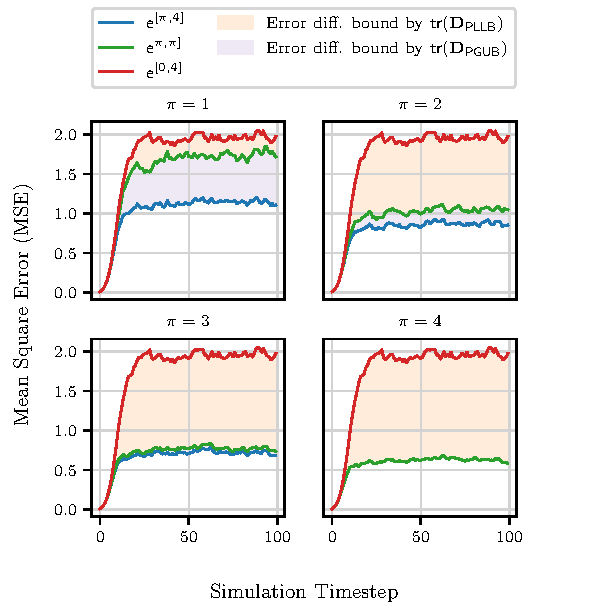
\includegraphics{figures/priv_estimation_fus_mse_privs.pdf}
  \caption{Average MSE of different estimators for $1000$ simulation runs when $V=2$ and $W=10$.}
  \label{fig:priv_estimation:fus_mse_privs}
\end{figure}

To demonstrate the effect of parameters $V$ and $W$ (and therefore $\mat{V}$ and $\mat{W}$), figure \ref{fig:priv_estimation:fus_mse_params} shows their effect on the MSE given fixed estimators. It can be seen that $V$ has a more prominent effect on the PLLB while $W$ has it on the PGUB. However, it can also be observed that both parameters affect both bounds to some degree, revealing some limitations when specific bounds are desired using the proposed scheme.
\begin{figure}[htbp]
  \centering
  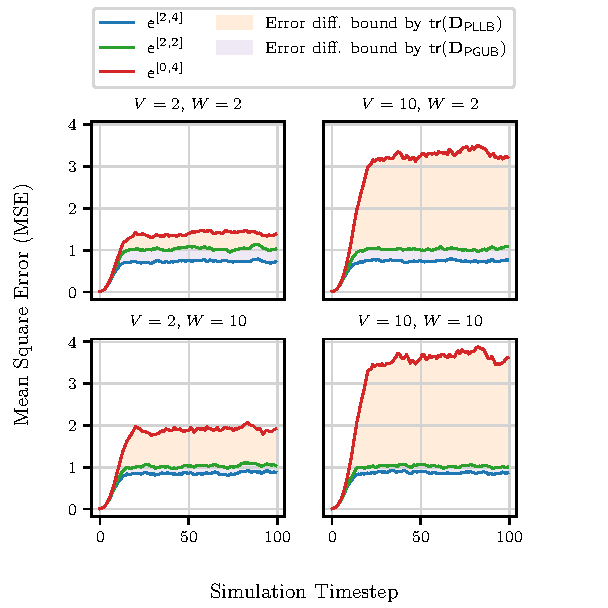
\includegraphics{figures/priv_estimation_fus_mse_params.pdf}
  \caption{Average MSE of unprivileged and privilege-$2$ estimators for $1000$ simulation runs when varying $V$ and $W$.}
  \label{fig:priv_estimation:fus_mse_params}
  % Variables, colours and sizes to look like others.
\end{figure}
Figure \ref{fig:priv_estimation:fus_trace_params} further captures this relation between the bounds and the parameters $V$ and $W$. As the simulated system is asymptotically stable, steady-state error covariances are reached as $k \to \infty$, and therefore $\mat{D}_{\mathsf{PLLB},k}$ and $\mat{D}_{\mathsf{PGUB},k}$ stabilise as well. From the figure, we can see that increasing the fully correlated noise parameter $V$ cannot greatly reduce the PGUB (\textit{i.e.}, bring $\mathsf{tr}(\mat{D}_{\mathsf{PGUB},k})$ closer to $0$), likely due to the accurate estimation of this component by privileged estimators and the remaining uncorrelated component staying unchanged. Simultaneously, however, the fully correlated component can greatly increase the PLLB (\textit{i.e.}, take $\mathsf{tr}(\mat{D}_{\mathsf{PLLB},k})$ further from $0$) as it increases the redundancy of fusing only unprivileged measurements. The effects of increasing $W$ are less one-sided. The PGUB is reduced due to sufficient uncorrelated noise making the fusion of unprivileged measurements hold little information even when some keys are known, but the PLLB is increased, as uncorrelated noise still affects estimators fusing only unprivileged measurements, albeit less drastically.

Figure \ref{fig:priv_estimation:fus_trace_params} also shows how the bounds are affected by the privilege $\pi$ they are computed for. Predictably, higher privilege results in fewer additional unprivileged measurements to fuse, lowering the PGUB but also producing better estimates for the privileged estimator, increasing the PLLB. We can also see that when the fully correlated noise term $V$ is small and privilege is low ($\pi=1$), unprivileged estimators with access to all measurements can perform better than privileged ones accessing only privileged measurements (resulting in a negative $\mathsf{tr}(\mat{D}_{\mathsf{PLLB},k})$).
\begin{figure}[htbp]
  \centering
  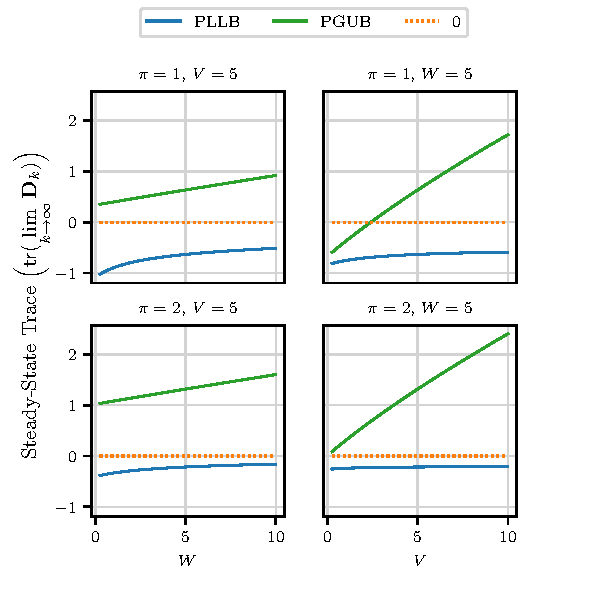
\includegraphics{figures/priv_estimation_fus_trace_params.pdf}
  \caption{Steady-state traces of the PLLB and PGUB for privileges $\pi=1$ and $\pi=2$ when $V$ and $W$ are varied.}
  \label{fig:priv_estimation:fus_trace_params}
  % Variables, colours and sizes to look like others.
\end{figure}

% 
%  .d8888b.   .d88888b.  888b    888  .d8888b.  
% d88P  Y88b d88P" "Y88b 8888b   888 d88P  Y88b 
% 888    888 888     888 88888b  888 888    888 
% 888        888     888 888Y88b 888 888        
% 888        888     888 888 Y88b888 888        
% 888    888 888     888 888  Y88888 888    888 
% Y88b  d88P Y88b. .d88P 888   Y8888 Y88b  d88P 
%  "Y8888P"   "Y88888P"  888    Y888  "Y8888P"  
%                                               
%                                               
%                                               
% 

\section{Conclusions on Provable Estimation Difference}\label{sec:priv_estimation:conclusion}
Tackling this problem, we have presented the idea of privileged estimation and given a formal cryptographic definition of covariance privilege that can be used to derive and prove an estimation performance difference between estimators with different properties. One free parameter allowed the magnitude of this difference to be controlled by the scheme designer. The extension to an environment with multiple sensors and multiple privileges was also considered, and two important privilege-dependent estimation performance differences were derived for which the same notion could also be used. Here, two free parameters loosely controlled the magnitudes of the differences but their complex relationship showed that more care needs to be taken when choosing them than in the single-sensor case. Both cases were analysed cryptographically and simulated to evaluate performance.

Future work on provable estimation performances includes hardware implementations to demonstrate real-time capability, finding independent free parameters in the multiple-sensor case and exploring methods for decentralised correlated noise generation with fewer communication costs.